\documentclass[aspectratio=169, 10pt, xcolor=table]{beamer}

% --- Package Configuration ---
\usepackage{booktabs}   % Table styling
\usepackage{tikz}       % Drawing
\usepackage{pgfgantt}   % Gantt charts in LaTeX
\usepackage{listings}   % Code listings
\usetikzlibrary{shapes, arrows.meta, positioning, fit, backgrounds, shadows, calc}

% --- Theme Settings: FU Berlin Style ---
\usetheme{Madrid}

% 1. Define FU Berlin Official Colors
\definecolor{FUblue}{RGB}{0, 51, 102}    % Dark Blue (Primary)
\definecolor{FUgreen}{RGB}{153, 204, 0}  % Bright Green (Accent)
\definecolor{FUgray}{RGB}{235, 235, 235} % Light Gray for backgrounds

% 2. Apply Structure Colors
\usecolortheme[named=FUblue]{structure} 

% 3. Specific Overrides for FU Look
\setbeamercolor{frametitle}{bg=FUblue, fg=white}
\setbeamercolor{framesubtitle}{fg=FUgreen}
\setbeamercolor{title}{bg=FUblue, fg=white}
\setbeamercolor{author}{fg=FUblue}
\setbeamercolor{institute}{fg=black}
\setbeamercolor{date}{fg=gray}
\setbeamercolor{block title}{bg=FUblue, fg=white}
\setbeamercolor{block body}{bg=FUblue!5, fg=black}

\rowcolors{2}{FUblue!5}{white}

% --- Custom Graphics Styles ---
\tikzset{
    basicbox/.style={
        rectangle, rounded corners, draw=FUblue!80, fill=white, 
        very thick, align=center, minimum height=0.8cm, drop shadow
    },
    arrow/.style={-{Stealth[length=3mm]}, thick, color=FUblue},
}

% --- Title Information ---
\title[Smart Home Demo Lab]{Smart Home Demo Lab\\Final Project Report}
\author[Team 2]{Yixue Wang, Linghao Dong, Yang Xiao, Chenxu Liu, Tong Lu}
\institute{Freie Universität Berlin}
\date{February 2026}

\begin{document}

% --- Slide 1: Title ---
\begin{frame}
    \titlepage
\end{frame}

% --- Slide 1.5: Team Intro ---
\begin{frame}{Meet the Team}
    {Smart Home Demo Lab - Team 2}
    
    \begin{columns}[c]
        \column{0.5\textwidth}
            \centering
            \textbf{\Large Team Members}
            \vspace{1em}
            
            \begin{itemize}[<+->]
                \item \textbf{Yixue Wang}
                \item \textbf{Linghao Dong}
                \item \textbf{Yang Xiao}
                \item \textbf{Chenxu Liu}
                \item \textbf{Tong Lu}
            \end{itemize}

        \column{0.5\textwidth}
            \centering
            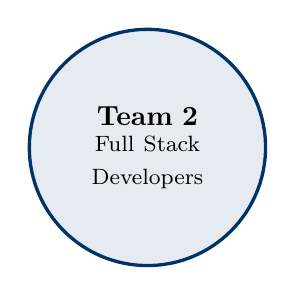
\begin{tikzpicture}
                \node[circle, draw=FUblue, fill=FUblue!10, very thick, minimum size=3cm, text width=2cm, align=center] {
                    \textbf{Team 2}\\
                    \footnotesize Full Stack\\Developers
                };
            \end{tikzpicture}
    \end{columns}
\end{frame}

% --- Slide 2: Motivation ---
\begin{frame}{Topic \& Project Motivation}
    {Smart Home Demo Lab - Team 2}

    \begin{block}{Topic}
        \textbf{Programmable Scene}: Define Automation Logic.
    \end{block}
    
    \pause
    \vspace{1em}
    
    \begin{block}{Project Motivation}
        \begin{itemize}[<+->]
            \item \textbf{Home Assistant}: Feature-heavy but overly complex.
            \item \textbf{Our Mission}: Simplify complexity while maintaining reliability.
        \end{itemize}
    \end{block}
\end{frame}

% --- Slide 3: Goals ---
\begin{frame}{Goals / Requirements}
    {Smart Home Demo Lab - Team 2}
    
    \begin{block}{Internal Goals / Requirements}
        \begin{itemize}[<+->]
            \item \textbf{Domain Driven Design (DDD) + Onion Architecture}: Independence
            \item \textbf{Extensibility}: Integration capabilities for new device and scenarios.
            \item \textbf{Testability}: Support for hardware mocking.
        \end{itemize}
    \end{block}

    \pause

    \begin{block}{External Goals / Requirements}
        \begin{itemize}[<+->]
            \item \textbf{Integration}: Interact with Home Assistant API.
            \item \textbf{Automation}: Trigger-Condition-Action model.
            \item \textbf{Usability}: Graphical Scene Editor (based on DAG style).
        \end{itemize}
    \end{block}
\end{frame}

% --- Slide 4: MVP ---
\begin{frame}{Minimum Viable Product (MVP)}
    {Smart Home Demo Lab - Team 2}
    
    \centering
    \begin{beamercolorbox}[sep=1em, rounded=true, shadow=true, wd=0.95\textwidth, center]{block body}
        \begin{itemize}[<+->]
            \setlength\itemsep{0.8em}
            \item \textbf{Device Management}: Device Registration, Status Monitoring and Control
            \item \textbf{Scenario Management}: Creation, save, and execution.
            \item \textbf{Automation Core}: Implementation of trigger, condition, action logic.
            \item \textbf{Frontend}: Interactive Visual Dashboard.
        \end{itemize}
    \end{beamercolorbox}
\end{frame}

% --- Slide 4: Implementation - Architecture ---
\begin{frame}{Implementation: Global Architecture}
    {Strict adherence to Onion Architecture for maintainability}
    
    \centering
    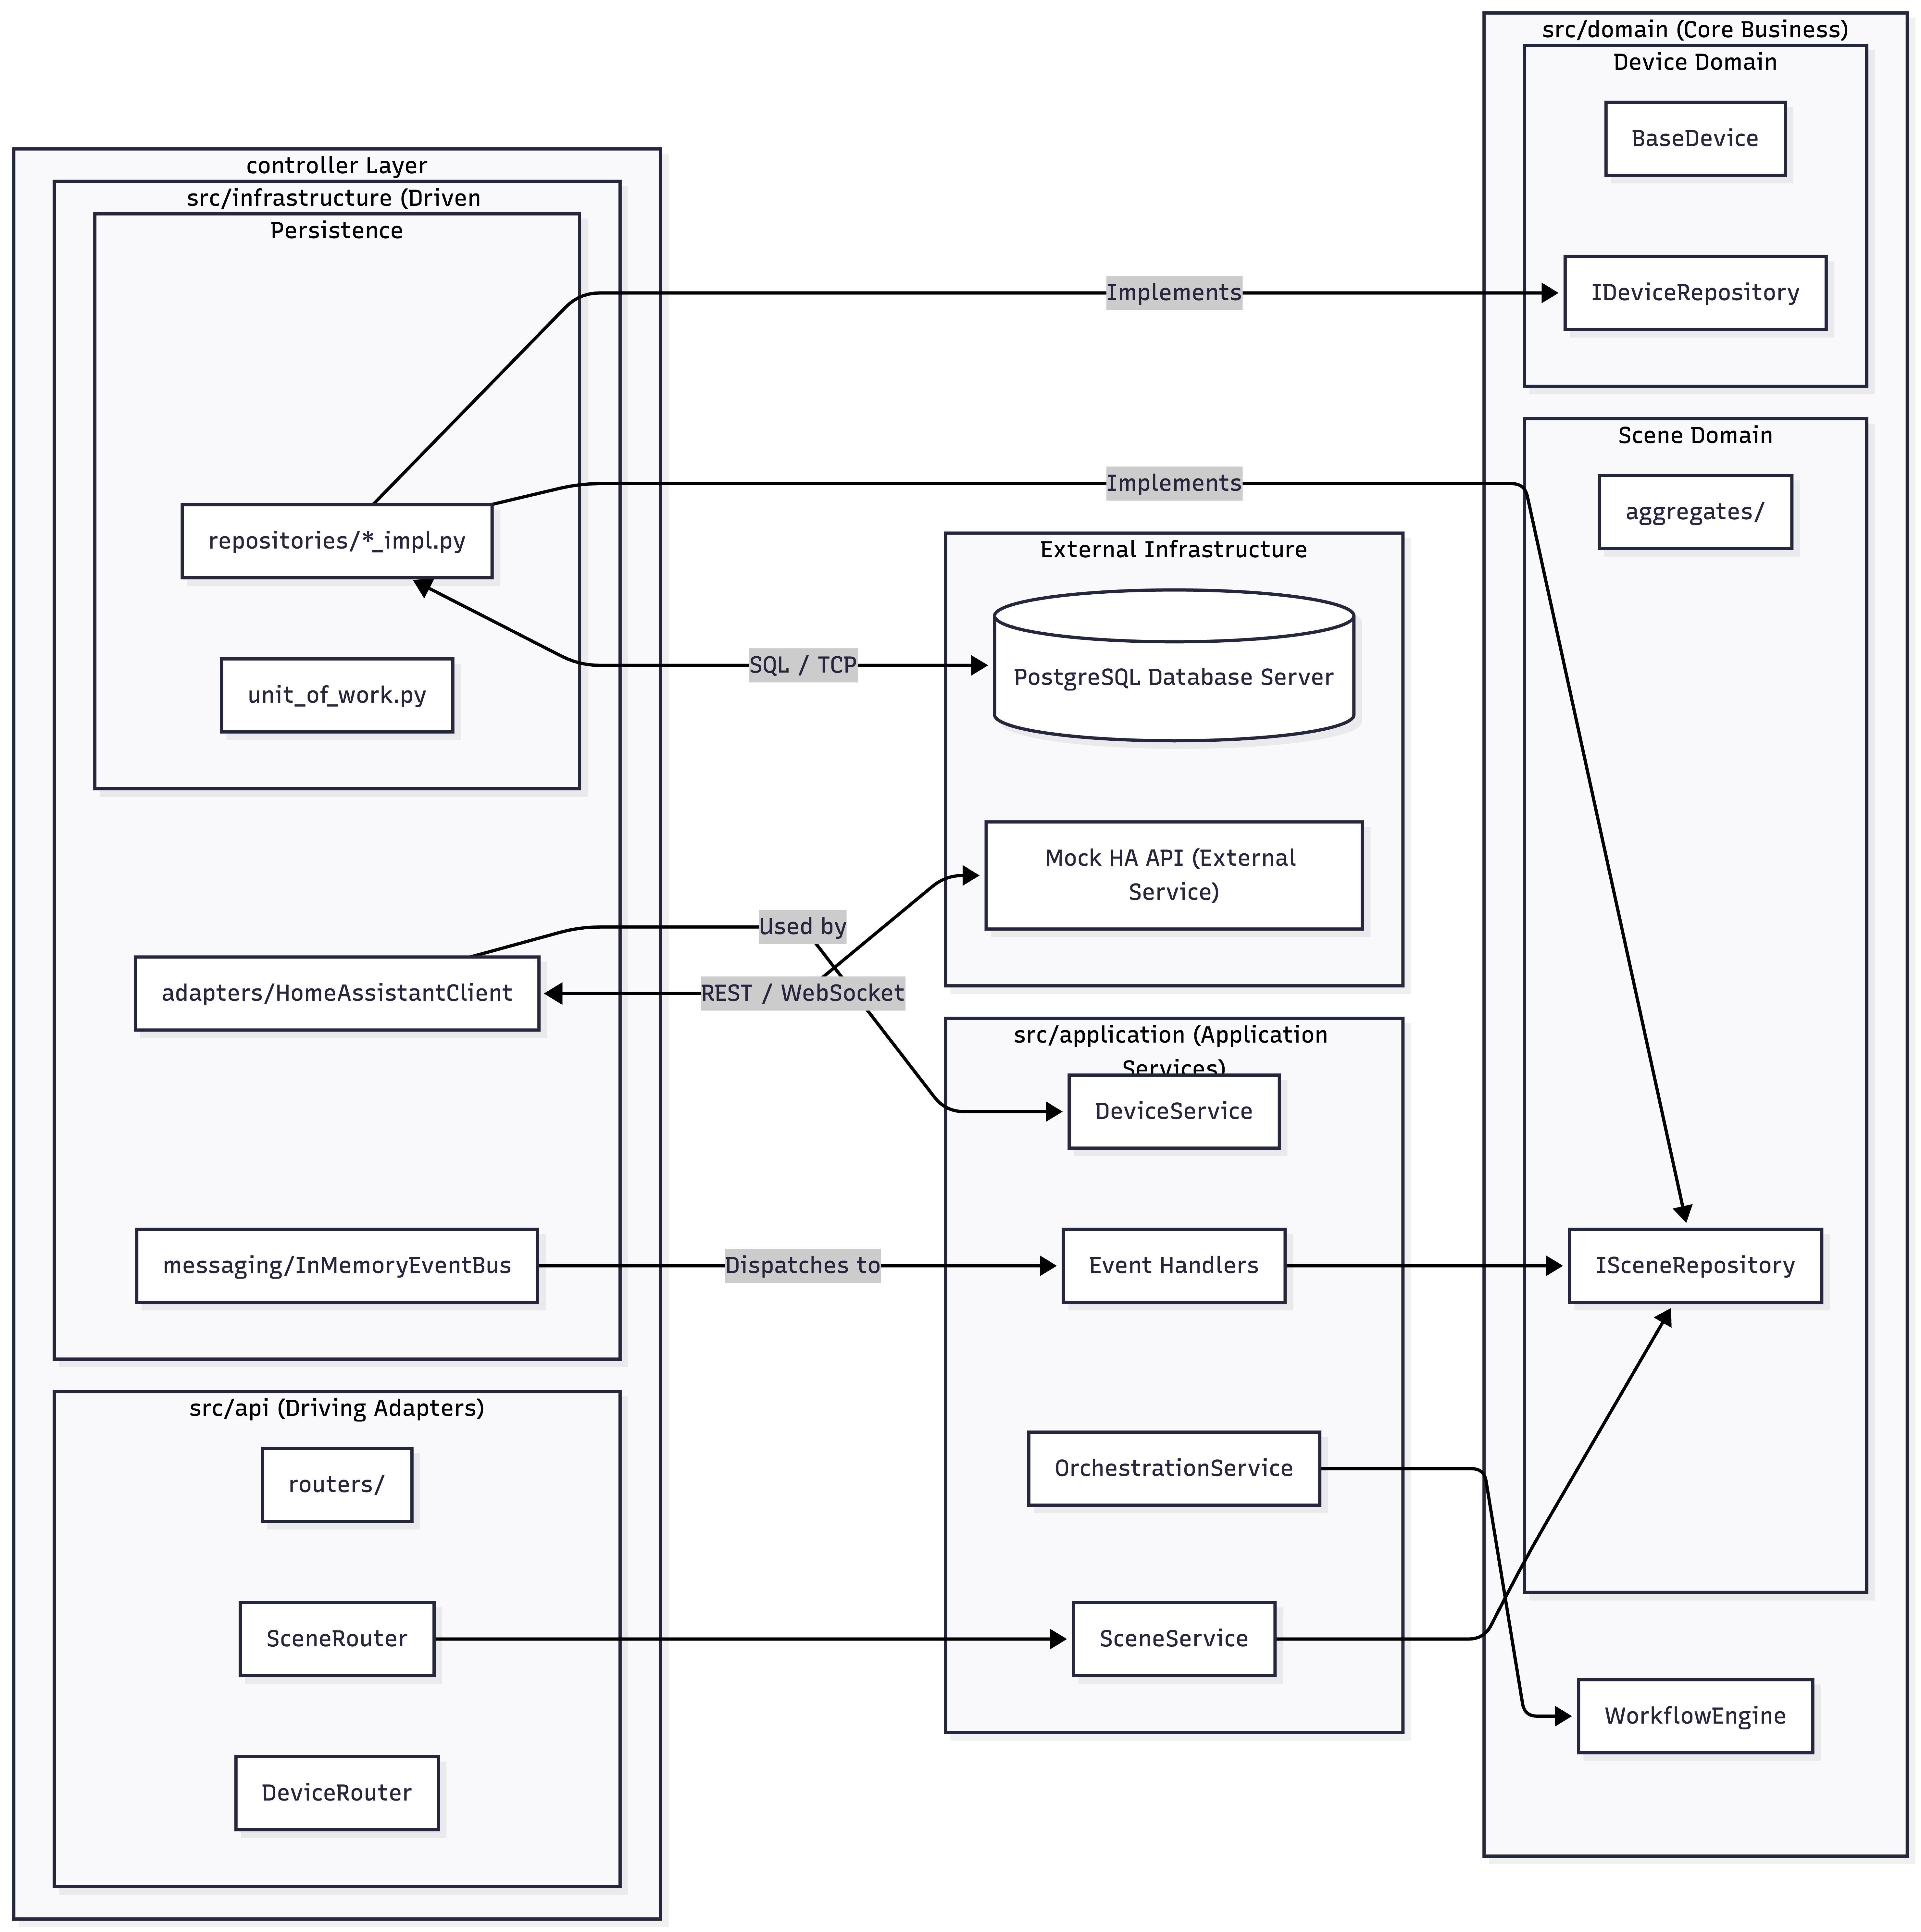
\includegraphics[width=0.45\textwidth]{3.1.png}
\end{frame}

% --- Slide 5: Tech Stack ---
\begin{frame}{Implementation: Technology Stack}
    {A professional implementation focusing on decoupling and scalability}

    % Top Row
    \begin{columns}[t]
        \column{0.48\textwidth}
            \begin{block}{Architecture \& Engineering}
                \begin{itemize}[<+->]
                    \item \textbf{Onion Arch \& DDD}: Strict \textbf{Layering} \& \textbf{Dependency Inversion}.
                    \item \textbf{Scalability}: Designed for high \textbf{extensibility} and modularity.
                    \item \textbf{Event-Driven}: Async Event Bus.
                \end{itemize}
            \end{block}

        \column{0.48\textwidth}
            \begin{block}{Frontend Visualization}
                \begin{itemize}[<+->]
                    \item \textbf{Visual Editor}: Custom DAG Engine (SVG/Canvas).
                    \item \textbf{Modern Stack}: React / Vite / Lucide.
                    \item \textbf{Custom UI}: Responsive Vanilla CSS system.
                \end{itemize}
            \end{block}
    \end{columns}

    \pause
    \vspace{0.2em}

    % Bottom Row
    \begin{columns}[t]
        \column{0.48\textwidth}
            \begin{block}{Backend Core}
                \begin{itemize}[<+->]
                    \item \textbf{FastAPI}: High-performance async service.
                    \item \textbf{Persistence}: SQLAlchemy + PostgreSQL.
                    \item \textbf{Scheduler}: APScheduler for automation logic.
                \end{itemize}
            \end{block}

        \column{0.48\textwidth}
            \begin{block}{Integration \& QA}
                \begin{itemize}[<+->]
                    \item \textbf{Hardware Abstraction}: Home Assistant REST API.
                    \item \textbf{Reliability}: Pytest-Asyncio / Mock Hardware.
                \end{itemize}
            \end{block}
    \end{columns}
\end{frame}


% --- Slide 6.5: Solution - UI ---
\begin{frame}{Solution: User Interface}
    {Visualization of the Smart Home Controller Dashboard}
    \centering
    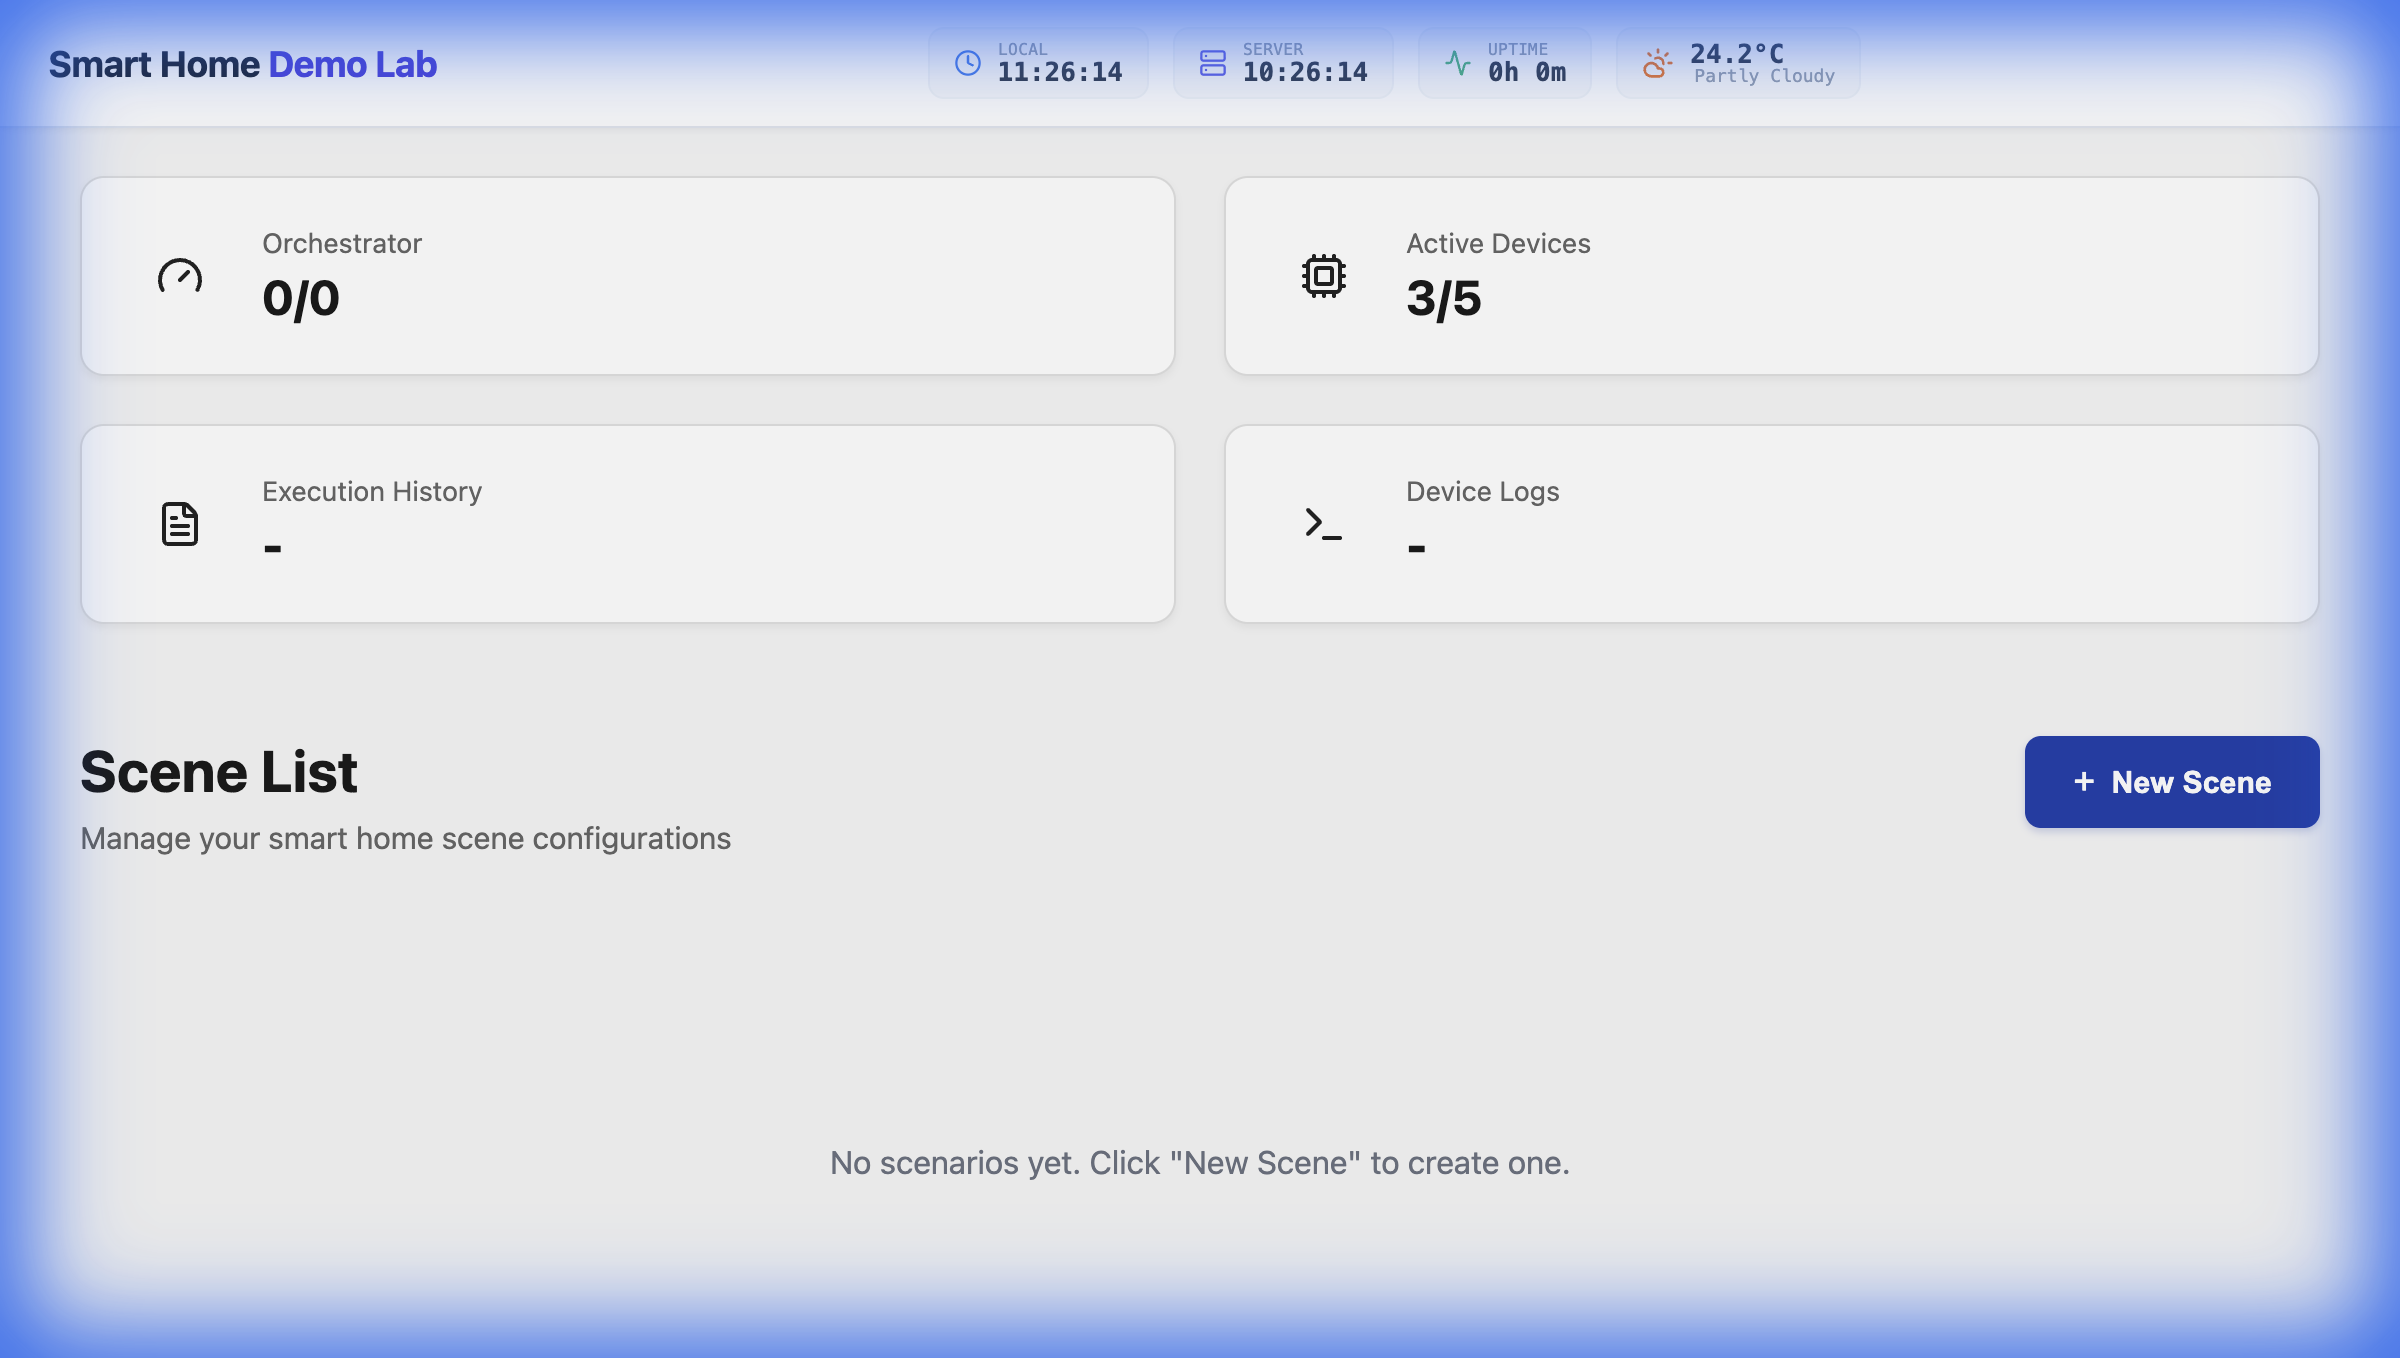
\includegraphics[width=0.80\textwidth]{ui_screenshot.png}

    \vspace{0.5em}
    \footnotesize
    \begin{itemize}[<+->]
        \item \textbf{Dashboard}: Real-time status of Device Aggregates.
        \item \textbf{Orchestration}: Visual feedback for Workflow execution.
    \end{itemize}
\end{frame}

% --- Slide 7: Timeline ---
\begin{frame}{Project Timeline}
    {From Planning to Final Delivery}
    \centering
    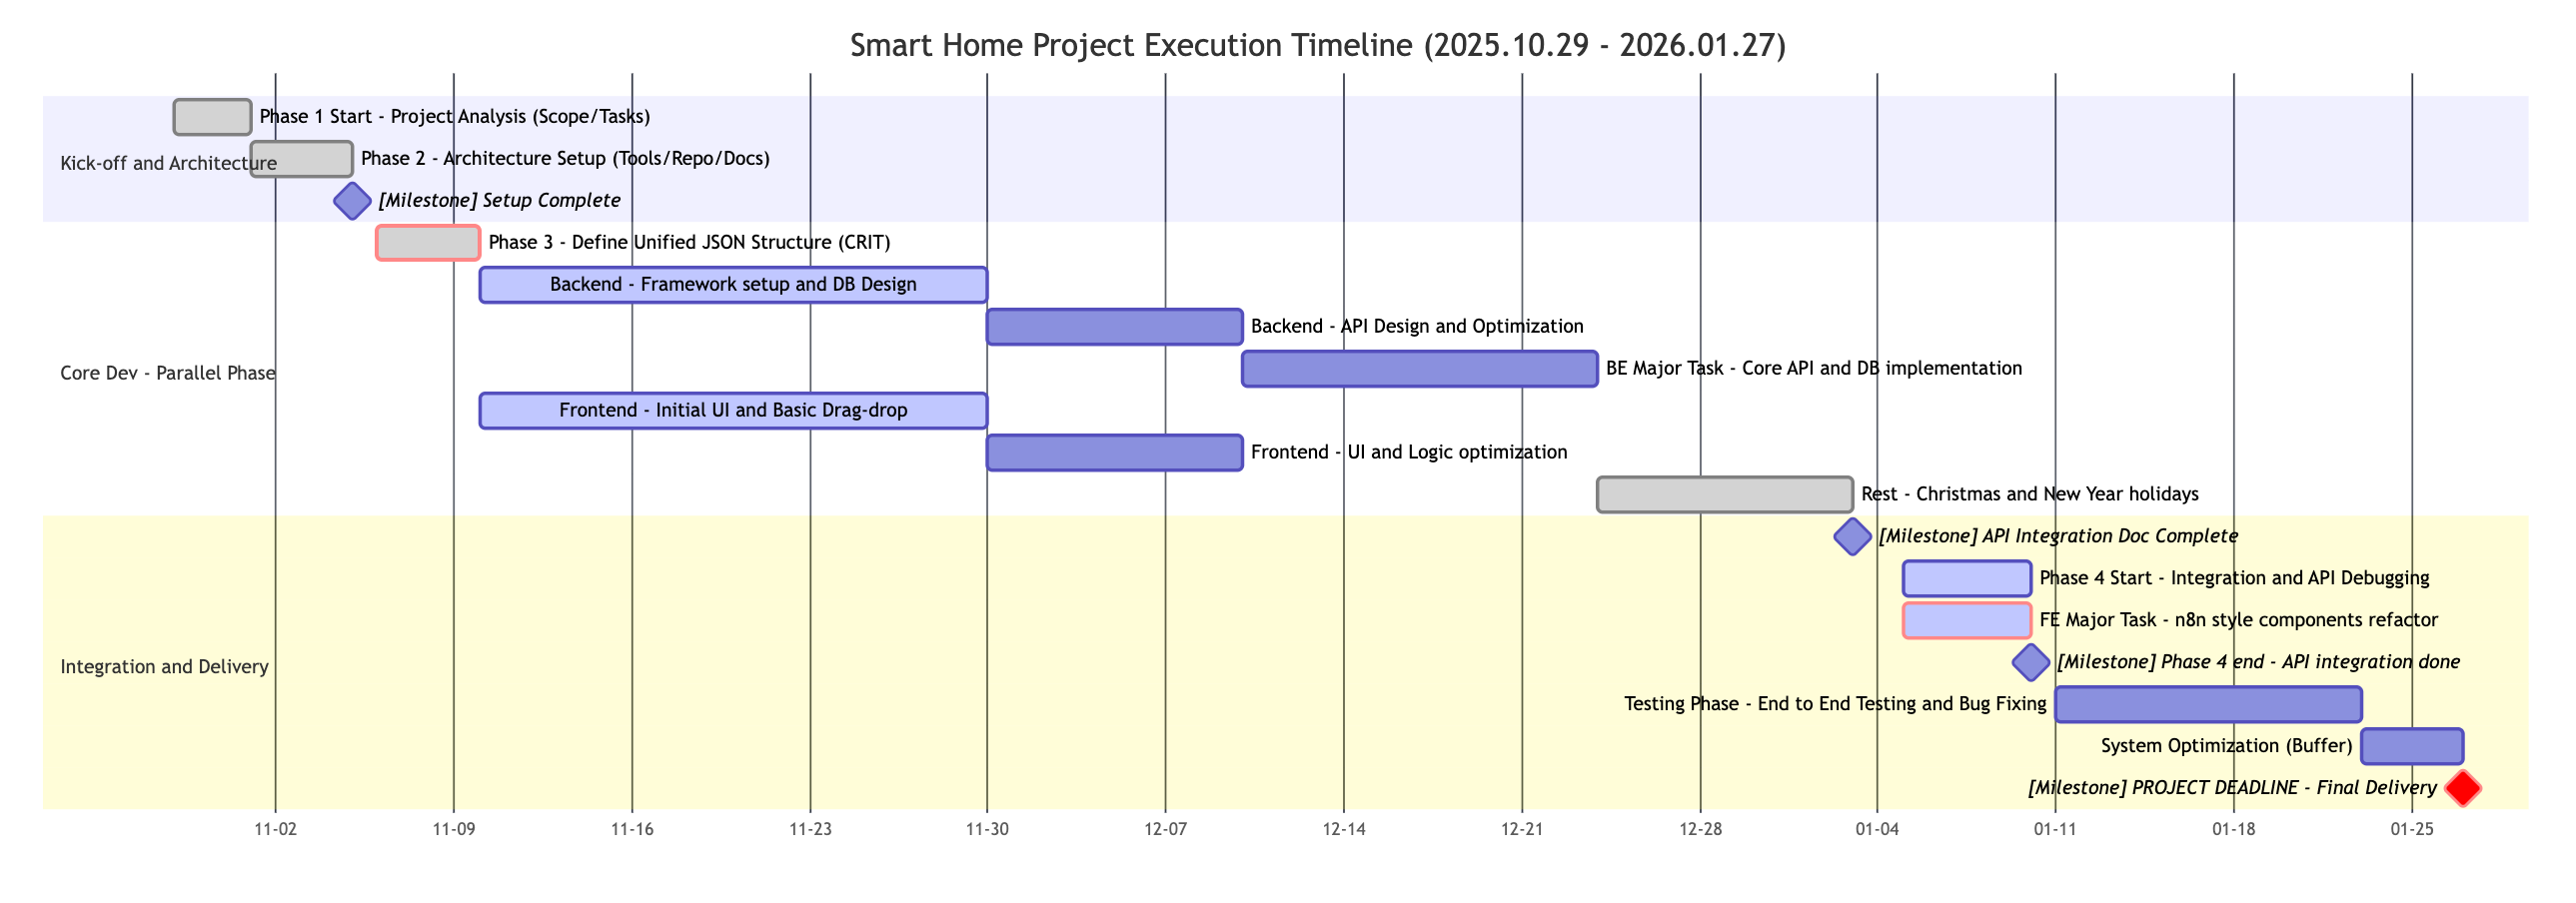
\includegraphics[width=0.95\textwidth]{timeline.png}
\end{frame}

% --- Slide 8: Conclusion ---
% --- Slide 8: System Data Flow (Moved) ---

% --- Slide 8: System Data Flow ---


% --- Slide 9: Conclusion ---
% --- Slide 9: Conclusion (Achievements) ---
\begin{frame}{Conclusion}
    {Project Summary \& Architectural Validation}
    
    \Large \color{FUblue} \textbf{What did we achieve?}
    \vspace{1em}
    \normalsize
    \begin{itemize}[<+->]
        \setlength\itemsep{1.5em}
        \item \textbf{Full-Stack Implementation}
        \item \textbf{Visual DAG Editor}
        \item \textbf{Hardware Simulation}
        \item \textbf{Complex Logic Solved}
    \end{itemize}
\end{frame}

% --- Slide 9.5: Conclusion (Conclusions Reached) ---
\begin{frame}{Conclusion}
    {Project Summary \& Architectural Validation}

    \Large \color{FUblue} \textbf{What conclusions did we reach?}
    \vspace{1em}
    \normalsize
    \begin{itemize}[<+->]
        \setlength\itemsep{1.5em}
        \item \textbf{Visualization is the only solution to complex logic.}
        \item \textbf{The importance of real-time.}
        \item \textbf{The system needs to provide real-time feedback on user actions.}
    \end{itemize}
\end{frame}

% --- Slide 10: Future Works (Feasibility) ---
\begin{frame}{Future Works: Roadmap to a "Security Lab"}
    {Transitioning from a Controller to a Research Testbed}
    \renewcommand{\arraystretch}{1.1} % Standardizing stretch
    \centering
    \footnotesize
    \begin{tabular}{l p{6cm} l}
        \toprule
        \textbf{Feature} & \textbf{Strategic Goal} & \textbf{Feasibility} \\
        \midrule
        \rowcolor{FUgray}
        \textbf{Auth \& Access} & Role-based Access Control (RBAC) \& TLS. & \textbf{High} \\
        \textbf{Scene Nesting} & Recursive logic for complex automation reuse. & \textbf{High} \\
        \rowcolor{FUgray}
        \textbf{Attack Actor} & Inject fault events and DoS simulations. & \textbf{Medium} \\
        \textbf{GenAI Config} & GenAI-driven intent understanding \& config generation. & \textbf{Medium} \\
        \rowcolor{FUgray}
        \textbf{Physical Testbed} & Real-world validation on physical hardware (no simulation). & \textbf{Low (Hard)} \\
        \bottomrule
    \end{tabular}
\end{frame}

% --- Slide 11: Reflection (Works/Not) ---
\begin{frame}{Reflection: Analysis of Outcomes}
    {Part 1: What worked well vs. What did not?}
    \footnotesize
    \begin{columns}[t]
        \column{0.5\textwidth}
            \begin{block}{What worked well? $\checkmark$}
                \pause
                \begin{itemize}[<+->]
                    \setlength\itemsep{0.5em}
                    \item \textbf{Strict Onion Architecture}: Strong decoupling allowed changing Infrastructure (e.g., DB) without touching Domain logic.
                    \item \textbf{API-First Design}: Defined Contracts (OpenAPI) first, enabling Frontend to develop without blocking on Backend.
                    \item \textbf{Mock Server}: Effectively decoupled development progress from unstable hardware availability.
                \end{itemize}
            \end{block}

        \column{0.5\textwidth}
            \begin{block}{What did NOT work? $\times$}
                \pause
                \begin{itemize}[<+->]
                    \setlength\itemsep{0.5em}
                    \item \textbf{Integration Timing}: "Big Bang" integration at the end caused hidden bugs (Leading to "Tracer Bullet" idea).
                    \item \textbf{Manual Object Mapping}: Tedious conversion between DTOs, Domain Entities, and ORM Models resulted in boilerplate.
                    \item \textbf{Over-Engineering}: Initial focus on "Perfect Architecture" detached us from actual User Scenarios.
                \end{itemize}
            \end{block}
    \end{columns}
\end{frame}

% --- Slide 12: What would do differently ---
\begin{frame}{What would we do differently next time?}
    {Part 2: Hypothetical Corrective Actions}
    \footnotesize
    \begin{columns}[c]
        \column{0.65\textwidth}
            \begin{itemize}[<+->]
                \setlength\itemsep{1.2em}
                
                \item \textbf{Process: "Tracer Bullet" Approach}
                \newline Build \textbf{vertically}: Implement one full feature (e.g., "Toggle Light") from UI to Hardware in Week 1 to validate the path.

                \item \textbf{Scope: Feature-First, Architecture-Second}
                \newline Implement core value (Attack Sim) first, refactor later. Don't start with heavy frameworks.

                \item \textbf{Testing: Real Hardware Earlier}
                \newline Mandate testing on simple hardware early (Week 2), rather than 100\% Mock Server until the end.
            \end{itemize}

        \column{0.35\textwidth}
            \centering
            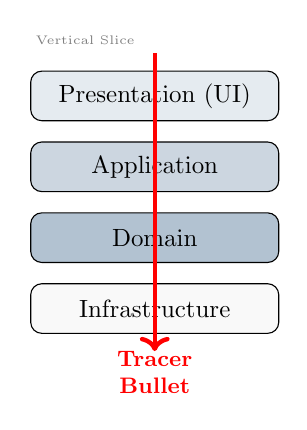
\begin{tikzpicture}[scale=0.9, transform shape]
                % Layers
                \node[draw, fill=FUblue!10, minimum width=3.5cm, minimum height=0.7cm, rounded corners] (ui) at (0, 3) {Presentation (UI)};
                \node[draw, fill=FUblue!20, minimum width=3.5cm, minimum height=0.7cm, rounded corners] (app) at (0, 2) {Application};
                \node[draw, fill=FUblue!30, minimum width=3.5cm, minimum height=0.7cm, rounded corners] (dom) at (0, 1) {Domain};
                \node[draw, fill=FUgray!30, minimum width=3.5cm, minimum height=0.7cm, rounded corners] (inf) at (0, 0) {Infrastructure};
                
                % Arrow
                \draw[->, ultra thick, red] (0, 3.6) -- (0, -0.6);
                \node[red, font=\bfseries\small, align=center] at (0, -0.9) {Tracer\\Bullet};
                
                % Annotation
                \node[anchor=south west, font=\tiny, color=gray] at (-1.8, 3.6) {Vertical Slice};
            \end{tikzpicture}
    \end{columns}
\end{frame}

% --- Slide 13: Lessons Learned ---
\begin{frame}{Lessons Learned}
    {Part 3: Key Takeaways for our Engineering Career}
    \footnotesize
    \pause
    \begin{block}{1. The Cost of Abstraction}
        Clean Architecture is powerful but expensive. For early-stage demos or MVPs, \textbf{YAGNI} (You Aren't Gonna Need It) should outweigh architectural purity.
    \end{block}

    \vspace{0.5em}
    \pause

    \begin{block}{2. The "Integration Tax"}
        Integration risks grow exponentially with time. Delaying integration until the end implies that you are creating a "debt" of unverified assumptions.
    \end{block}

    \vspace{0.5em}
    \pause

    \begin{block}{3. Contracts set you Free}
        Investing time in a strict \textbf{JSON Schema/OpenAPI} at the very beginning was the single best decision we made. It allowed 5
         people to work in parallel without blocking.
    \end{block}
\end{frame}

% --- Slide 11: Thank You ---
\begin{frame}
    \centering
    \Huge \color{FUblue} \textbf{Thank You!}
    
    \vspace{1cm}
    \normalsize
    \textbf{Questions?}
    
    \vspace{2cm}

\end{frame}

\end{document}
